\documentclass[12pt,a4paper]{article}

\usepackage[margin=1in]{geometry}
\usepackage{amsmath}
\usepackage{amssymb}
\usepackage{booktabs}
\usepackage{graphicx}
\usepackage{natbib}
\usepackage{setspace}
\usepackage{hyperref}
\usepackage{array}
\usepackage{threeparttable}
\usepackage{lscape}
\usepackage{float}
\usepackage{multirow}
\usepackage{tabularx}
\usepackage{caption}

\onehalfspacing

\title{Forecasting Foreign Exchange Reserves For Sri Lanka : A multivariate time series approach}

\author{}

\date{}

\begin{document}

\maketitle

\begin{abstract}
This paper compares classical econometric, Bayesian, regime-switching, and machine-learning models for forecasting Sri Lanka's foreign exchange reserves over 2005--2025, including the 2022 sovereign default episode. Using rolling-origin evaluation across five variable sets, we find that Markov-Switching VAR in a disaggregated balance-of-payments specification delivers the strongest point-forecast performance, reducing RMSE by roughly three-quarters relative to a random-walk benchmark in the post-default window. A factorial decomposition shows that model architecture explains more of this gain than simply expanding the information set, and that balance-of-payments disaggregation is most effective when paired with regime-switching structure. These results support regime-aware, component-level reserve forecasting as a practical framework for policy surveillance in crisis-prone emerging markets.

\noindent\textbf{Keywords:} Foreign exchange reserves, forecasting, Markov-switching VAR, balance of payments disaggregation, regime dynamics, machine learning, Sri Lanka, sovereign default, emerging markets

\noindent\textbf{JEL Classification:} C52, C53, E47, F31, F37
\end{abstract}

\section{Introduction}

For emerging market economies, adequate foreign exchange reserves serve as the primary defence against balance-of-payments crises, currency runs, and sovereign debt distress \citep{JeanneRanciere2011}. Sri Lanka's experience between 2019 and 2022 underscores this point. Gross reserves declined from approximately US\$7.6 billion at end-2019 to an estimated US\$50 million of usable reserves by April 2022, precipitating the country's first sovereign default since independence \citep{Athukorala2024}. GDP contracted by more than 7\%, inflation surpassed 50\%, and widespread social upheaval toppled the sitting government \citep{Weerakoon2023}.

Despite this policy relevance, reserve forecasting has attracted considerably less academic attention than exchange rate prediction, inflation forecasting, or GDP nowcasting \citep{Rossi2013}. Existing contributions are largely confined to single-model frameworks \citep{SehgalSharma2008,Gosselin2005} and rarely assess performance across structural breaks. No existing study benchmarks classical, Bayesian, regime-switching, and machine learning approaches on identical data with formal statistical comparison, or evaluates forecast accuracy through a sovereign default episode.

This paper has three objectives. First, it compares the out-of-sample accuracy of classical econometric, Bayesian, regime-switching, and machine learning models for reserve forecasting, evaluated on a dataset spanning stable accumulation, pandemic disruption, sovereign default, and IMF-supervised recovery. Second, it decomposes the relative contributions of model architecture and information content through a factorial design. Third, it provides a component-level scenario framework for policy surveillance, with quantified sensitivity to currency, trade, and programme disbursement shocks.

The analysis evaluates twelve model specifications across five variable sets of increasing dimensionality, using rolling-origin backtests with expanding estimation windows. A temporally motivated train-validation-test split isolates pre-crisis (through 2019), crisis (2020--2022), and post-default (2023--2025) regimes. Model comparisons are formalised through \cite{DieboldMariano1995} tests and the Model Confidence Set of \cite{HansenLundeNason2011}.

The main findings are as follows. MS-VAR achieves RMSE reductions of 74--77\% relative to the na\"{\i}ve benchmark in the parsimonious and BoP specifications. A factorial decomposition shows that model architecture accounts for the bulk of this gain. Aggregating balance-of-payments flows into net flows destroys approximately 94\% of the gross flow signal. The Meese-Rogoff puzzle does not hold in its strong form: MS-VAR outperforms the random walk even during the acute crisis segment. Diagnostic analysis of regime persistence, impulse response asymmetry, and classification certainty provides analytical evidence for the sources of this advantage.

The paper contributes to three areas. Empirically, it provides the first comparison of classical, Bayesian, regime-switching, and machine learning reserve forecasting approaches evaluated through a sovereign default, addressing a gap in the literature where forecast accuracy has been tested only during stable periods. Methodologically, it introduces a factorial decomposition of architecture and information effects and a formal test for information loss under flow aggregation. For policy, it contributes a scenario analysis framework applicable to central bank reserve management and IMF surveillance.

\section{Background and Literature Review}

\subsection{From Adequacy Ratios to Dynamic Forecasting}

The reserve adequacy literature has produced a series of static threshold metrics: import-cover rules, the Guidotti-Greenspan ratio \citep{Greenspan1999}, monetary-based benchmarks \citep{Calvo1996,Wijnholds2001}, and the IMF's composite Assessing Reserve Adequacy (ARA) framework \citep{IMF2011,IMF2015}. \cite{Obstfeld2010} shifted attention to financial-sector liabilities as the relevant scale variable, while \cite{JeanneRanciere2011} formalised the cost-benefit calculus of reserve holdings.

These frameworks share a fundamental limitation: they assess reserve \textit{levels} against static benchmarks rather than forecasting reserve \textit{trajectories}. Static ratios cannot anticipate the speed of depletion, the timing of threshold breaches, or the state-dependent dynamics that accelerate crises. Early warning systems \citep{KaminskyLizondoReinhart1998,FrankelSaravelos2012} partially address this gap by predicting binary crisis events, but they do not produce the continuous reserve path forecasts needed for operational policy planning. Dynamic forecasting models are therefore a necessary complement to adequacy ratios, particularly in settings where reserves can decline rapidly across regime boundaries.

Two further features of reserve dynamics complicate static approaches. First, reserves are actively managed policy variables, not passive residuals of balance-of-payments accounting. \cite{AizenmanLee2007} distinguished precautionary motives (buffering against sudden stops) from mercantilist motives (supporting export competitiveness), each generating different accumulation dynamics and depletion vulnerabilities. Second, the marginal value of reserves is highly nonlinear: negligible when buffers are large, but very high near the critical zone where market confidence collapses \citep{JeanneRanciere2011}. This threshold nonlinearity implies that linear models are misspecified near crisis points, because the relationship between reserves and their determinants changes qualitatively with the reserve level itself.

\subsection{Reserve Forecasting Literature}

Table~\ref{tab:lit_summary} summarises the key contributions to the reserve forecasting literature. Several patterns are evident. First, the literature is sparse relative to exchange rate or inflation forecasting. Second, nearly all studies evaluate performance during stable accumulation periods; none systematically assesses accuracy through a sovereign default. Third, the literature predominantly treats reserves as a scalar aggregate, ignoring the compositional dynamics of underlying balance-of-payments flows.

\begin{table}[htbp]
\centering
\caption{Summary of Reserve Forecasting Literature}
\label{tab:lit_summary}
\begin{tabular}{p{3.2cm}p{2.2cm}p{3cm}p{1.5cm}p{3.5cm}}
\toprule
Study & Country & Method(s) & Crisis? & Key Finding \\
\midrule
\cite{SehgalSharma2008} & India & ARIMA & No & Reasonable in-sample fit; limited out-of-sample reliability \\
\cite{Gosselin2005} & 12 EM & Panel ECM & No & Long-run relationships hold; model breaks down in crises \\
\cite{Gupta2014} & China & DMA, DMS, BMA & No & DMS outperforms linear models; time-varying weights matter more than predictor expansion \\
\cite{Salas2025} & 102 countries & BMA-Na\"{\i}ve Bayes & No & Strong classification accuracy; no sovereign default evaluation \\
This paper & Sri Lanka & MS-VAR, BVAR, XGBoost, DMA, + others & Yes & Regime-switching dominates; architecture matters more than information \\
\bottomrule
\end{tabular}
\begin{tablenotes}
\small
\item \textit{Notes:} EM = Emerging Markets. ``Crisis?'' indicates whether the evaluation window includes a sovereign default or comparable episode.
\end{tablenotes}
\end{table}

\cite{SehgalSharma2008} applied ARIMA models to Indian reserves and found acceptable in-sample fit but limited out-of-sample reliability. A key limitation is the univariate framework, which cannot capture the multivariate dynamics of balance-of-payments components. \cite{Gosselin2005} extended the approach to a panel error-correction framework across twelve economies, documenting cointegrating relationships between reserves, imports, and short-term debt. However, their model broke down during crisis episodes, highlighting the central challenge that forecast accuracy is most needed when it is hardest to achieve. \cite{Gupta2014} applied DMA and DMS to Chinese reserves and found that time-varying model weights outperform both linear models and static model averaging. Their result that adaptive model composition matters more than predictor expansion motivates the inclusion of DMA and DMS in the present study. \cite{Salas2025} applied BMA across 102 countries with strong classification results, but did not evaluate performance through a sovereign default.

Machine learning methods have shown competitive results in adjacent forecasting problems \citep{MedeirosVasconcelosVeigaZilberman2021,RichardsonMulderVehbi2021}, yet their systematic application to reserve forecasting remains limited. The broader evidence suggests that machine learning offers its greatest advantage in stable periods with strong nonlinear patterns, while simpler approaches often dominate during structural breaks \citep{RichardsonMulderVehbi2021}.

\subsection{Methodological Foundations}

The Meese-Rogoff result \citep{MeeseRogoff1983} established that structural exchange rate models cannot outperform a random walk out of sample. This finding has proved robust across currencies and time periods \citep{Rossi2013,CheungChinnPascual2005}. Reserves are driven by many of the same balance-of-payments fundamentals and exhibit similar nonlinearities. \cite{TaylorPeelSarno2001} argued that nonlinear mean reversion becomes detectable when deviations from fundamentals are large, suggesting that the puzzle may weaken during strong directional trends.

The Markov-switching framework \citep{Hamilton1989,Krolzig1997} is particularly suited to this setting because it allows all model parameters to shift between discrete states. \cite{Peria2002} and \cite{BrunettiMarianoScottiTan2007} applied Markov-switching models to speculative attacks in European and Southeast Asian settings, but neither applied the framework to reserve forecasting with disaggregated balance-of-payments flows. Bayesian VARs with Minnesota priors \citep{Litterman1986,Banbura2010} address the curse of dimensionality through informative shrinkage, while DMA and DMS \citep{Raftery2010,KoopKorobilis2012} allow model weights to evolve over time. Gradient-boosted trees \citep{ChenGuestrin2016} and LSTM networks \citep{HochreiterSchmidhuber1997} offer flexible nonlinear alternatives, though their performance is sensitive to hyperparameter choices and training set size.

Three gaps in this literature motivate the present study. First, no existing comparison jointly evaluates classical, Bayesian, regime-switching, and machine learning approaches for reserve forecasting on identical data and evaluation criteria. Second, regime-switching models have not been applied to disaggregated balance-of-payments components in a reserve forecasting context. Third, systematic evaluation through a sovereign default is absent. \cite{Gupta2014} demonstrated the value of DMA and DMS for reserve forecasting with linear constituent models; the present study extends their approach by incorporating regime-switching specifications into the DMA/DMS model pool, testing whether dynamic combination of regime-aware and linear forecasts yields further gains.

Based on the theoretical considerations and empirical gaps identified above, this paper tests three hypotheses. (H1) Regime-switching models outperform linear and machine learning alternatives for reserve forecasting in a sample that includes a sovereign default. (H2) Model architecture (regime-switching versus linear/tree-based) explains more of the forecast accuracy differential than information content (parsimonious versus disaggregated variable sets). (H3) Aggregating gross balance-of-payments flows into net flows destroys predictive information through cancellation of offsetting components.

\subsection{The Sri Lankan Reserve Crisis}

Sri Lanka's gross reserves declined from approximately US\$7.6 billion at end-2019 to an estimated US\$50 million of usable reserves by April 2022, when the government suspended external debt service \citep{Athukorala2024}. The decline was driven by tourism revenue loss (COVID-19 and the 2019 Easter attacks), fiscal deterioration, and a Central Bank policy of defending the pegged exchange rate through reserve sales. Between September 2021 and March 2022 alone, gross reserves fell from US\$3.1 billion to under US\$2 billion. An IMF Extended Fund Facility (US\$2.9 billion) was approved in March 2023, and by early 2024 gross reserves had rebuilt to approximately US\$4.4 billion \citep{Weerakoon2023,UNDP2022}.

This chronology generates a reserve series with at least three distinct regimes: gradual accumulation (2005--2019), rapid depletion (2020--2022), and post-default rebuilding (2023 onward). Each regime exhibits different dynamics, volatility, and relationships to driving variables. Bai-Perron multiple structural break tests applied to the gross reserves series identify five significant breaks (2009:10, 2014:04, 2017:05, 2020:02, 2022:04), confirming the regime structure that motivates the emphasis on Markov-switching specifications.

\section{Data and Variable Construction}

\subsection{Data Sources and Sample}

The dataset comprises nine monthly time series spanning January 2005 to December 2025 (252 observations), drawn from the Central Bank of Sri Lanka (CBSL) statistical database, the IMF's International Reserves and Foreign Currency Liquidity (IRFCL) template, the Colombo Stock Exchange market statistics, and Sri Lanka Customs trade returns. All monetary variables are denominated in US dollars to ensure comparability and to avoid conflating real dynamics with exchange rate valuation effects. Table~\ref{tab:descriptive} reports descriptive statistics for all series.

\begin{table}[htbp]
\centering
\caption{Descriptive Statistics of Key Variables}
\label{tab:descriptive}
\begin{tabular}{lrrrrr}
\toprule
Variable & Obs & Mean & Std Dev & Min & Max \\
\midrule
Gross Reserves (USD m) & 252 & 5450.6 & 2105.4 & 1588.4 & 9935.8 \\
Exports (USD m) & 224 & 886.8 & 176.8 & 282.3 & 1302.2 \\
Imports (USD m) & 225 & 1487.3 & 315.8 & 606.3 & 2241.0 \\
Trade Balance (USD m) & 224 & $-$601.1 & 227.8 & $-$1100.6 & $-$39.1 \\
Remittances (USD m) & 202 & 507.8 & 121.8 & 204.9 & 812.7 \\
Tourism (USD m) & 192 & 171.4 & 128.0 & 0.0 & 475.2 \\
Exchange Rate (LKR/USD) & 228 & 177.0 & 77.3 & 107.6 & 363.3 \\
M2 (USD m) & 225 & 25436.4 & 12829.8 & 7095.5 & 48091.1 \\
CSE Net Flows (USD m) & 166 & 3.6 & 26.3 & $-$62.2 & 143.8 \\
\bottomrule
\end{tabular}
\begin{tablenotes}
\small
\item \textit{Sample period: 2005-01 to 2025-12 (252 months).} Exchange rate expressed as LKR per USD.
\end{tablenotes}
\end{table}

\subsection{Dependent Variable}

Gross official reserves (USD millions) constitute the primary dependent variable, serving as the numerator of every major adequacy benchmark \citep{JeanneRanciere2011,Obstfeld2010}. Joint ADF and KPSS testing confirms that gross reserves are integrated of order one. The first-differenced series (reserve change) is therefore the primary forecast target for the regime-switching systems. For MS-VAR and MS-VECM, predicted changes are mapped back to levels by cumulative summation from the last observed reserve level. The na\"{\i}ve benchmark is a random walk in levels, $\hat{y}_{t+h|t}=y_t$ for all $h$. All reported point metrics (RMSE, MAE, MAPE, MASE) are computed on level forecasts against observed levels for every model, including the benchmark, ensuring an identical target scale. The first-differenced series exhibits a negative first-order autocorrelation (ACF(1) = $-0.301$), indicating mean-reverting intervention behaviour that differs between accumulation and crisis regimes.

Official reserve data from the CBSL statistical database and the IMF's IRFCL template are subject to minimal measurement error relative to forecast uncertainty, as they reflect audited central bank balance sheet positions. We do not model measurement error explicitly but note that any such error would attenuate estimated forecast accuracy differences, making the reported performance gaps conservative.

\subsection{Variable Set Design}

Five variable sets of increasing dimensionality are defined to disentangle the effect of model specification from the effect of information content. This design is motivated by the well-documented tension in small-sample macroeconomic forecasting between information gains from additional predictors and estimation error from parameter proliferation \citep{Banbura2010,Carriero2015}. By evaluating each model across all five sets, the analysis identifies whether forecast failures stem from model misspecification or from over- or under-parameterisation.

\begin{table}[htbp]
\centering
\caption{Variable Set Specifications and Effective Samples}
\label{tab:varsets}
\begin{tabular}{llcc}
\toprule
Variable Set & Key Variables & $k$ & Effective Coverage \\
\midrule
Parsimonious & Reserves, trade balance, exchange rate & 3 & 2007:01--2025:12 \\
BoP & Reserves, exports, imports, remittances, tourism & 5 & 2009:01--2025:03 \\
Monetary & Reserves, exchange rate, M2 & 3 & 2005:01--2025:06 \\
PCA & Reserves + 3 PCs from 8 indicators & 4 & 2012:01--2024:11 \\
Full & All available predictors & 9 & 2012:01--2025:03 \\
\bottomrule
\end{tabular}
\begin{tablenotes}
\small
\item \textit{Notes:} $k$ = number of endogenous variables in the VAR system. Missing-data handling follows a uniform rule before evaluation: forward-fill up to 3 consecutive months (matching the quarterly reporting frequency of several source series), then drop remaining missing rows. No model-specific imputation is used in the horse-race stage. The BoP set replaces trade balance with separate exports and imports to identify independent shocks. The PCA set extracts three principal components from eight indicators, fitted on training data only to avoid look-ahead bias.
\end{tablenotes}
\end{table}

The \textbf{Parsimonious set} ($k=3$: reserves, trade balance, exchange rate) captures the first-order determinants of reserve dynamics under the import-cover and exchange rate defence frameworks. The trade balance, computed as FOB exports minus CIF imports, serves as the aggregate current account proxy. The USD/LKR exchange rate is fundamentally endogenous to reserve dynamics under Sri Lanka's managed float, since central bank intervention to defend the peg directly depletes reserves \citep{Obstfeld2010}.

The \textbf{Balance of Payments set} ($k=5$) disaggregates the current account into exports, imports, remittances, and tourism earnings alongside reserves. The disaggregation is driven by the requirements of the MS-VAR framework, which needs to identify independent shocks to each flow component. This is critical because BoP components exhibit sharply divergent crisis dynamics: during the 2020--2022 period, exports and imports moved in opposite directions, whilst remittances and tourism followed distinct structural break patterns.

The \textbf{Monetary set} ($k=3$) comprises reserves, the exchange rate, and broad money (M2), introducing the domestic capital flight channel identified by \cite{Obstfeld2010} and captured in the IMF's ARA metric. This compact specification tests whether monetary aggregates provide incremental forecasting power beyond trade flows.

The \textbf{PCA set} ($k=4$) comprises reserves plus three principal components extracted from the eight indicators in the broader dataset. This tests whether dimensionality reduction can preserve informational content while reducing estimation burden. The approach is particularly relevant for the BVAR and MS-VAR specifications, where parameter proliferation in small samples is a binding constraint. The three retained components explain 79.5\% of total variance (PC1: 46.1\%, PC2: 20.8\%, PC3: 12.7\%).

The \textbf{Full set} ($k=9$) includes all available predictors simultaneously. It serves as an upper bound on available information and as a test of whether regularisation mechanisms (Minnesota shrinkage, tree-based feature selection, LSTM dropout) can effectively manage the dimensionality.

Table~\ref{tab:varsets} highlights the ragged-edge implications of uneven source coverage: variable sets are estimated on different effective windows, but all models within a given variable set are evaluated on the same preprocessed sample. Cross-model comparisons within a variable set are therefore sample-aligned; cross-variable-set comparisons should be interpreted with the effective-sample caveat in mind.

\subsection{Stationarity and Seasonal Properties}

All series are subjected to joint ADF and KPSS testing to determine the order of integration. Variables confirmed as I(1) are first-differenced for VAR estimation; where cointegrating relationships are identified via the Johansen procedure, the VECM specification is estimated in levels with error-correction terms. Seasonal properties are assessed via STL decomposition. Variables exhibiting seasonal strength above 0.5---notably tourism earnings (0.593)---are deseasonalised using X-13ARIMA-SEATS prior to estimation in specifications that do not include seasonal dummies.

\section{Methodology}

\subsection{Model Overview}

The model set spans classical econometrics (ARIMA, VAR, VECM), regime-switching specifications (MS-VAR, MS-VECM), Bayesian approaches (BVAR), dynamic model combination (DMA, DMS), machine learning (XGBoost, LSTM, XGB-Quantile), and na\"{\i}ve benchmarks (random walk, seasonal na\"{\i}ve). Additional specifications include a balance-of-payments identity model (BoPIdentity) and a local-level stochastic volatility model (LocalLevelSV). All models are estimated in an expanding-window fashion, initialising on the training period (January 2005--December 2019, 180 observations) and expanding monthly through the validation (2020--2022) and test (2023--2025) periods. Standard estimation details are reported in Appendix~A.

This section focuses on the non-standard modelling choices that distinguish the present application from textbook implementations.

\subsection{Regime-Switching Specifications}

The MS-VAR allows all parameters to shift between two discrete regimes (accumulation and depletion) governed by an unobserved Markov chain with state $S_t \in \{0, 1\}$:
\[
\mathbf{y}_t = \mathbf{c}_{S_t} + \sum_{i=1}^{p} \mathbf{A}_{i,S_t} \mathbf{y}_{t-i} + \mathbf{u}_t, \quad \mathbf{u}_t \sim \mathcal{N}(\mathbf{0}, \boldsymbol{\Sigma}_{S_t})
\]
Parameters are estimated via the EM algorithm. The key modelling choice is the two-regime specification, motivated by the distinct accumulation and depletion dynamics visible in the reserve series. Higher-order specifications ($K = 3$) were explored but yielded poorly identified regimes with short durations, consistent with the limited within-regime observations available in a 252-month sample. At the default iteration cap, some full-sample runs can stop at the maximum iteration bound; accordingly, the regime diagnostics are complemented with a seeded multi-start stability check under a higher iteration cap (Section~\ref{sec:regime_char}).

For the MS-VECM extension, a critical design decision concerns the cointegrating vectors:
\[
\Delta \mathbf{y}_t = \boldsymbol{\alpha}_{S_t} \boldsymbol{\beta}' \mathbf{y}_{t-1} + \sum_{i=1}^{p-1} \boldsymbol{\Gamma}_{i,S_t} \Delta \mathbf{y}_{t-i} + \mathbf{u}_t
\]
The cointegrating vectors $\boldsymbol{\beta}$ are estimated on the full sample and held regime-invariant, whilst the adjustment speeds $\boldsymbol{\alpha}_{S_t}$ and short-run dynamics $\boldsymbol{\Gamma}_{i,S_t}$ are regime-dependent. This follows the approach of \cite{Krolzig1997}: the long-run equilibrium between reserves, trade flows, and the exchange rate is assumed to hold across regimes, but the speed at which the system corrects deviations from equilibrium differs between accumulation and crisis states.

\subsection{XGBoost Rolling Feature Engineering}

The XGBoost implementation departs from standard applications through its rolling feature engineering pipeline, which constructs 3-month and 6-month rolling means and volatility estimates for all variables at each forecast origin. This creates a feature set that evolves with the expanding estimation window, capturing momentum and volatility clustering that are economically meaningful for reserve dynamics. The rolling construction ensures that no future information leaks into the feature set. XGB-Quantile extends the framework to produce probabilistic forecasts by predicting the 10th, 25th, 50th, 75th, and 90th percentiles of the conditional distribution. Time-series cross-validation tuning is employed for XGBoost in the parsimonious and BoP specifications, though robustness is mixed across folds.

\subsection{Architecture-vs-Information Factorial Decomposition}

A key methodological contribution is the formal disentangling of architecture (model class) from information content (variable set). We construct a 2$\times$2 factorial design crossing model class $\mathcal{M} \in \{\text{MS-VAR}, \text{XGBoost}\}$ with information set $\mathcal{I} \in \{\text{Parsimonious}, \text{BoP}\}$. For RMSE outcomes $R_{m,i}$, the architecture effect (holding information constant) is:
\[
\hat{\alpha} = \frac{1}{2}\sum_{i \in \mathcal{I}} \left[ R_{\text{XGB},i} - R_{\text{MSVAR},i} \right].
\]
The information effect (holding model constant) is:
\[
\hat{\iota} = \frac{1}{2}\sum_{m \in \mathcal{M}} \left[ R_{m,\text{Parsim}} - R_{m,\text{BoP}} \right].
\]
The interaction term captures whether the effect of information depends on architecture:
\[
\hat{\delta} = \left(R_{\text{XGB,Parsim}} - R_{\text{XGB,BoP}}\right) - \left(R_{\text{MSVAR,Parsim}} - R_{\text{MSVAR,BoP}}\right).
\]
This decomposition follows a standard two-factor analysis of variance structure applied to out-of-sample RMSE. It quantifies whether the MS-VAR advantage is driven primarily by regime-switching architecture, by richer information in disaggregated flows, or by the interaction between the two. The decomposition is descriptive rather than causal: it isolates the marginal contribution of each factor within the observed comparison set, but does not identify treatment effects in the econometric sense.

\subsection{Dynamic Model Averaging and Selection}

Dynamic Model Averaging and Dynamic Model Selection \citep{Raftery2010,KoopKorobilis2012} address model uncertainty by allowing the weights on competing forecasts to evolve over time. At each forecast origin $t$, DMA computes a posterior model probability $\pi_{t|t-1,k}$ for each constituent model $k$ and forms the combined forecast as the probability-weighted average. DMS selects the single model with the highest $\pi_{t|t-1,k}$. The forgetting factor $\alpha$ governs how quickly past performance is discounted. We set $\alpha = 0.99$, following the convention in \cite{KoopKorobilis2012}, implying an effective memory of roughly 100 periods. The rolling forecast-error variance is estimated over a 24-month window, chosen to span approximately two years of monthly data and thus capture medium-term shifts in relative model performance.

The constituent model pool comprises all seven non-DMA/DMS models evaluated on the BoP specification: ARIMA, BVAR, MS-VAR, MS-VECM, Na\"{\i}ve, VECM, and XGBoost. This design allows DMA and DMS to shift weight toward regime-switching models during crisis periods and toward simpler specifications during tranquil periods, an adaptive strategy that static model selection cannot replicate.

\subsection{Information Loss Under Aggregation}

To test whether aggregating balance-of-payments components into composite variables destroys predictive information, we formalise the aggregation mapping. Let $\mathbf{X}_t = (x_{1t}, \ldots, x_{kt})'$ denote the vector of gross BoP flows and $A_t = \mathbf{w}'\mathbf{X}_t$ the scalar aggregate (e.g., trade balance = exports $-$ imports). Forecasting with $A_t$ conditions on a strictly coarser $\sigma$-field than forecasting with $\mathbf{X}_t$, implying potential information loss. We quantify the empirical severity of this loss through a cancellation index:
\[
\text{CI}_t = \frac{|A_t|}{\sum_{j=1}^{k} |x_{jt}|},
\]
which measures the ratio of the net flow to the sum of absolute gross flows. When $\text{CI}_t$ is near zero, large gross flows cancel almost entirely, and the aggregate retains almost no information about the underlying dynamics.

\subsection{Evaluation Framework}

Forecasts at horizons $h \in \{1, 3, 6, 12\}$ months are evaluated using RMSE, MAE, MAPE, and MASE \citep{HyndmanKoehler2006} for point accuracy. Density forecasts are evaluated using CRPS and prediction interval coverage probability (PICP) at the 80\% and 95\% levels. An asymmetric policy loss function penalises under-prediction of reserve depletion at twice the rate of over-prediction (2:1 weight ratio), motivated by the observation that under-prediction of depletion carries higher policy costs than over-prediction, since responses to false alarms are inexpensive relative to the cost of undetected crises. All metrics are computed on reserve levels, with the random-walk benchmark transformed identically to the structural models.

Statistical significance is assessed via the \cite{DieboldMariano1995} test of equal predictive accuracy (with Harvey-Leybourne-Newbold small-sample correction) and the Model Confidence Set of \cite{HansenLundeNason2011}. The MCS uses a stationary block bootstrap with 1,000 replications and block length $\lceil T^{1/3} \rceil$, where $T$ is the number of forecast observations. Formal definitions of all metrics are provided in Appendix~A.

\section{Empirical Results}

\subsection{Main Forecasting Comparison}

\begin{figure}[htbp]
\centering
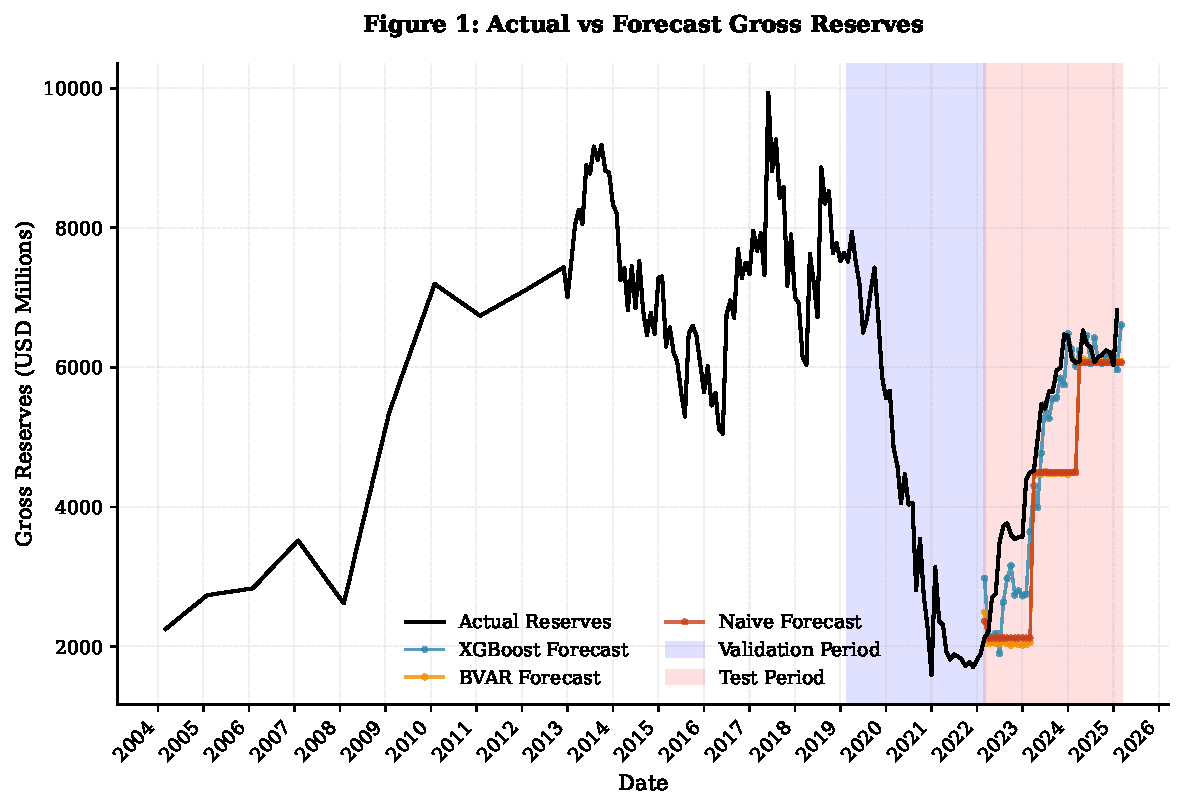
\includegraphics[width=\textwidth]{figures/figure_1_actual_vs_forecast.pdf}
\caption{Actual gross reserves and one-step-ahead forecasts from selected models. The validation period (2020--2022, blue shading) covers the pandemic and sovereign default; the test period (2023--2025, red shading) covers the IMF-supervised recovery.}
\label{fig:actual_vs_forecast}
\end{figure}

\begin{table}[htbp]
\centering
\caption{Out-of-Sample Forecast Accuracy: Parsimonious Specification, $h = 1$}
\label{tab:main_accuracy}
\begin{tabular}{lrrrrrrr}
\toprule
Model & RMSE & MAE & MAPE & MASE & Policy Loss & CRPS & $n$ \\
\midrule
\textbf{MS-VAR} & \textbf{311.8} & \textbf{230.3} & \textbf{5.20} & \textbf{0.77} & \textbf{408.4} & -- & 36 \\
MS-VECM & 357.7 & 280.5 & 6.31 & 0.94 & 512.7 & -- & 36 \\
XGBoost & 640.6 & 475.7 & 11.82 & 1.59 & 900.8 & 466.4 & 36 \\
XGB-Quantile & 655.5 & 521.8 & 12.25 & 1.75 & 1018.0 & 241.0 & 36 \\
ARIMA & 1170.4 & 896.2 & 21.61 & 3.00 & 1785.6 & 734.2 & 36 \\
Na\"{\i}ve & 1178.9 & 935.9 & 20.47 & 3.14 & 1864.2 & 761.5 & 36 \\
VECM & 1194.5 & 956.8 & 21.64 & 3.21 & 1892.3 & 782.4 & 36 \\
BVAR & 1214.9 & 964.4 & 21.41 & 3.23 & 1917.2 & 792.1 & 36 \\
\bottomrule
\end{tabular}
\begin{tablenotes}
\small
\item \textit{Notes:} MAPE in \%. Policy Loss = asymmetric loss ($2\times$ penalty for under-prediction). CRPS = Continuous Ranked Probability Score. Bold indicates best performance. Test period: 2023:01--2025:12. Dashes indicate models without probabilistic output in this specification.
\end{tablenotes}
\end{table}

Table~\ref{tab:main_accuracy} presents out-of-sample forecast accuracy for the parsimonious specification at $h=1$ over the test period (2023:01--2025:12). MS-VAR achieves RMSE of 311.8, versus 1,178.9 for the na\"{\i}ve random walk, a 73.6\% improvement. This advantage is consistent across all metrics: MAE of 230.3 (versus 935.9), MAPE of 5.20\% (versus 20.47\%), and MASE of 0.77, which falls below the 1.0 threshold indicating improvement over the na\"{\i}ve in-sample benchmark. MS-VECM follows at 357.7.

XGBoost achieves RMSE of 640.6. This is better than all classical and Bayesian specifications, but roughly double the MS-VAR error. Classical models (ARIMA, VECM) cluster in the range 1,170--1,195, performing no better than the na\"{\i}ve benchmark. BVAR achieves 1,214.9, reflecting the difficulty of estimating a high-dimensional system with limited pre-crisis training data.

Two distinct performance tiers emerge: regime-switching models (RMSE 312--358) and all others (RMSE $>$ 640). This gap motivates the diagnostic investigation in Section~\ref{sec:mechanism}.

\subsection{Statistical Significance}
\label{sec:stat_tests}

\begin{table}[htbp]
\centering
\caption{Diebold-Mariano Test Results: Selected Model Pairs}
\label{tab:dm_tests}
\begin{tabular}{lrl}
\toprule
Model Pair & DM $p$-value & Significance \\
\midrule
MS-VAR vs.\ ARIMA & 0.0006 & *** \\
MS-VAR vs.\ BVAR & $<$0.0001 & *** \\
MS-VAR vs.\ VECM & $<$0.0001 & *** \\
MS-VAR vs.\ Na\"{\i}ve & $<$0.0001 & *** \\
MS-VAR vs.\ XGBoost & 0.0012 & ** \\
MS-VECM vs.\ XGBoost & 0.0033 & ** \\
XGBoost vs.\ ARIMA & 0.0052 & ** \\
\bottomrule
\end{tabular}
\begin{tablenotes}
\small
\item \textit{Notes:} Diebold-Mariano test with Harvey-Leybourne-Newbold small-sample correction. Two-sided $p$-values. ***: $p < 0.001$; **: $p < 0.01$. Pairwise matrix totals cited in the text refer to the nine-model BoP specification, where the effective $h=1$ test window is 2023:01--2025:03 ($n=27$).
\end{tablenotes}
\end{table}

Table~\ref{tab:dm_tests} reports Diebold-Mariano tests for key model pairs. MS-VAR's advantage over all non-regime-switching, non-combination models is highly significant ($p < 0.01$ in every case). The MS-VAR vs.\ XGBoost comparison yields $p = 0.0012$, confirming that the regime-switching advantage is not a statistical artefact. Across the full nine-model set in the BoP specification (including DMA and DMS), 30 of 36 pairwise DM comparisons are significant at the 10\% level, and 28 at the 1\% level.

The Model Confidence Set at $\alpha = 0.10$ retains four models: MS-VAR, DMA, MS-VECM, and DMS. All five remaining models are eliminated: XGBoost ($p = 0.009$), ARIMA, Na\"{\i}ve, BVAR, and VECM (all $p < 0.001$). The MCS does not single out one winner. Instead, it draws a boundary between regime-aware methods (including dynamic combinations that lean heavily on regime-switching constituents) and all other specifications.

These inference results should be interpreted with appropriate caution. The BoP test window contains 27 effective monthly observations at $h=1$. Overlapping multi-step horizons further reduce effective independence (roughly $n_{\text{eff}} \approx n/h$: about 9 at $h=3$, 4--5 at $h=6$, and 2--3 at $h=12$). In short samples, both DM asymptotics and block-bootstrap MCS outcomes are sensitive to tuning choices such as block length. We therefore treat p-values as complementary evidence and place primary weight on rank stability and economic magnitude. In the BoP $h=1$ test window, MS-VAR lowers RMSE from 1,350.8 (na\"{\i}ve) to 315.2, a reduction of 1,035.6 USD million, approximately 22.3\% of mean test-period reserves.

\subsection{Horizon Sensitivity}

\begin{table}[htbp]
\centering
\caption{Forecast Accuracy Across Horizons: RMSE (Parsimonious Specification)}
\label{tab:horizon}
\begin{tabular}{lrrrrc}
\toprule
Model & $h = 1$ & $h = 3$ & $h = 6$ & $h = 12$ & $h_{12}/h_1$ \\
\midrule
XGBoost & \textbf{640.6} & \textbf{1281.7} & 1887.6 & 2664.2 & 4.16 \\
Na\"{\i}ve & 1178.9 & 1393.2 & \textbf{1737.4} & \textbf{2373.7} & 2.01 \\
VECM & 1194.5 & 1404.6 & 1751.5 & 2398.4 & 2.01 \\
BVAR & 1214.9 & 1438.0 & 1793.5 & 2488.9 & 2.05 \\
XGB-Quantile & 655.5 & 1384.5 & 1991.1 & 3095.0 & 4.72 \\
ARIMA & 1170.4 & 1561.6 & 2453.0 & 3444.6 & 2.94 \\
\bottomrule
\end{tabular}
\begin{tablenotes}
\small
\item \textit{Notes:} $h_{12}/h_1$ = deterioration ratio from 1-month to 12-month horizon. Bold indicates best performance at each horizon. Test period: 2023--2025. Parsimonious MS-VAR and MS-VECM horizon results are omitted here to avoid duplication with Table~\ref{tab:bop_horizon}, which reports the preferred BoP regime-switching specification used for the main regime comparisons.
\end{tablenotes}
\end{table}

Table~\ref{tab:horizon} reveals pronounced horizon dependence among non-regime-switching models. XGBoost dominates at short horizons ($h=1$: 640.6; $h=3$: 1,281.7). But this advantage deteriorates. By $h=6$, the na\"{\i}ve random walk (1,737.4) overtakes XGBoost (1,887.6). The pattern reflects a limitation of machine learning in macroeconomic forecasting: the model exploits patterns in the recent training distribution, and distributional shift erodes that advantage at longer horizons. Bayesian methods maintain more stable relative performance. BVAR's deterioration ratio is 2.05 versus 4.16 for XGBoost, reflecting the regularising benefit of the Minnesota prior.

\subsection{Validation versus Test Period}

\begin{table}[htbp]
\centering
\caption{Forecast Performance: Crisis Validation vs.\ Post-Default Test Period}
\label{tab:val_vs_test}
\begin{tabular}{lrrr@{\hskip 12pt}rrr}
\toprule
& \multicolumn{3}{c}{Validation (2020--2022)} & \multicolumn{3}{c}{Test (2023--2025)} \\
\cmidrule(lr){2-4} \cmidrule(lr){5-7}
Model & RMSE & MAE & MAPE & RMSE & MAE & MAPE \\
\midrule
XGBoost & 1183.5 & 1037.3 & 37.82 & 640.6 & 475.7 & 11.82 \\
XGB-Quantile & 1055.3 & 884.8 & 32.81 & 655.5 & 521.8 & 12.25 \\
ARIMA & 1986.3 & 1723.7 & 70.36 & 1170.4 & 896.2 & 21.61 \\
Na\"{\i}ve & 1328.1 & 1029.3 & 35.69 & 1178.9 & 935.9 & 20.47 \\
VECM & 1532.2 & 1289.6 & 46.57 & 1194.5 & 956.8 & 21.64 \\
BVAR & 1412.7 & 1128.9 & 39.59 & 1214.9 & 964.4 & 21.41 \\
\bottomrule
\end{tabular}
\begin{tablenotes}
\small
\item \textit{Notes:} Validation period coincides with the Sri Lankan economic crisis and sovereign default (April 2022). Test period covers the post-default recovery under the IMF Extended Fund Facility. MAPE in \%. This table focuses on the non-regime-switching parsimonious set; MS-VAR and MS-VECM period splits are reported in the BoP-focused regime tables to avoid repetitive presentation across specifications.
\end{tablenotes}
\end{table}

Table~\ref{tab:val_vs_test} stratifies results by the crisis validation period (2020:01--2022:12) and post-default test period (2023:01--2025:12). During the acute crisis, MAPE ranges from 33\% to over 70\% across these non-regime-switching models, indicating severe forecasting difficulty. In sharp contrast, during the post-crisis recovery, XGBoost achieves MAPE of 11.82\%, and multiple models achieve MAPE in the 20--22\% range. However, the regime-switching models---which are not shown in this parsimonious-only comparison but dominate the BoP results below---substantially outperform even during the crisis segment, as discussed in Section~\ref{sec:crisis_segment}.

\subsection{Balance of Payments Specification Results}

\begin{figure}[htbp]
\centering
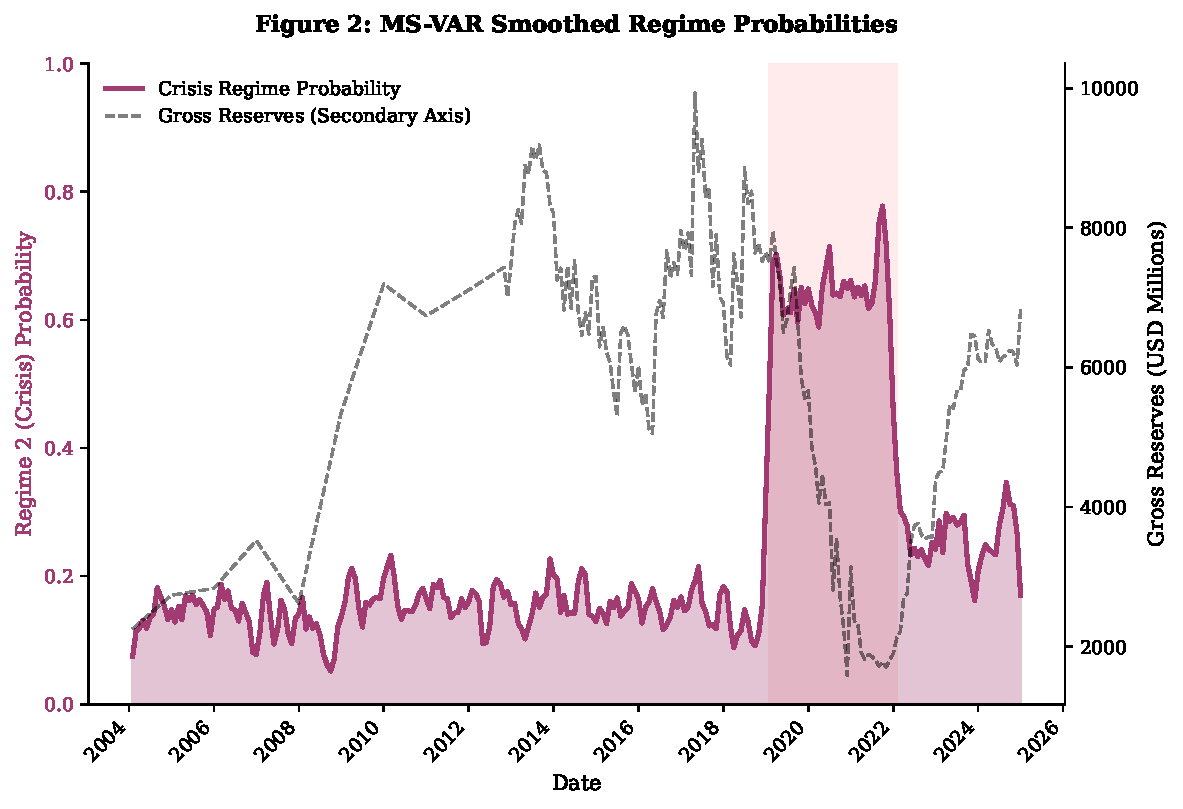
\includegraphics[width=\textwidth]{figures/figure_2_regime_probabilities.pdf}
\caption{MS-VAR smoothed regime probabilities (top axis) and actual gross reserves (bottom axis). The estimated crisis regime probability rises sharply during 2020--2022, consistent with the pandemic disruption and sovereign default, and recedes during the post-2023 IMF-supervised recovery.}
\label{fig:regime_probs}
\end{figure}

\begin{table}[htbp]
\centering
\caption{Forecast Accuracy Across Horizons: RMSE (Balance of Payments Specification)}
\label{tab:bop_horizon}
\begin{tabular}{lrrrr}
\toprule
Model & $h = 1$ & $h = 3$ & $h = 6$ & $h = 12$ \\
\midrule
\textbf{MS-VAR} & \textbf{315.2} & \textbf{679.5} & 1150.7 & 2050.4 \\
DMA & 321.7 & 694.2 & 1143.8 & 2031.5 \\
MS-VECM & 323.4 & 842.8 & 1697.0 & 3249.8 \\
DMS & 326.0 & 701.8 & \textbf{1049.8} & 2018.3 \\
LSTM & 479.7 & 713.9 & 1057.3 & \textbf{1742.2} \\
XGBoost & 886.1 & 1376.1 & 1869.4 & 2679.0 \\
BoPIdentity & 1136.4 & 1006.3 & 1169.6 & 2734.7 \\
ARIMA & 1249.9 & 1463.9 & 1834.0 & 2448.6 \\
Na\"{\i}ve & 1350.8 & 1599.9 & 1914.3 & 2541.6 \\
BVAR & 1361.5 & 1597.3 & 1888.6 & 2487.1 \\
LocalLevelSV & 1410.0 & 1661.9 & 1964.2 & 2569.3 \\
VECM & 1556.3 & 1601.3 & 1921.3 & 2650.5 \\
\bottomrule
\end{tabular}
\begin{tablenotes}
\small
\item \textit{Notes:} BoP set: reserves, exports, imports, remittances, tourism ($k=5$). DMA and DMS combine forecasts from all non-combination models in this specification. Test period: 2023--2025. Bold indicates best at each horizon.
\end{tablenotes}
\end{table}

Table~\ref{tab:bop_horizon} reveals a tight cluster of regime-aware models at the top of the BoP specification. MS-VAR achieves RMSE of 315.2 at $h=1$---a 76.7\% improvement over the na\"{\i}ve benchmark (1,350.8). DMA follows at 321.7, MS-VECM at 323.4, and DMS at 326.0. The gap separating these four models from the next competitor is large: XGBoost, at 886.1, trails by more than 560 RMSE points. At longer horizons, DMS becomes increasingly competitive ($h=6$: 1,049.8), and LSTM emerges as the strongest performer at $h=12$ (1,742.2), suggesting that both dynamic model selection and sequence models can capture longer-range dependencies that static regime-switching specifications miss.

The pattern is revealing. DMA and DMS succeed not by inventing new information, but by dynamically reweighting the constituent models. During periods when the MS-VAR dominates, DMA assigns it the lion's share of weight. When no single model clearly leads, the combination hedge pays off. The net result is a forecast that is nearly as accurate as the best individual model at short horizons and more robust across horizons.

The success of regime-aware methods on disaggregated BoP data points to a broader pattern. Accurate reserve forecasting benefits from separately modelling the distinct dynamics of each balance-of-payments component (exports, imports, remittances, tourism) and allowing those relationships to shift across economic states. The parsimonious specification, which aggregates exports and imports into a single trade balance, discards information about asymmetric crisis dynamics that regime-switching models can exploit.

\subsection{Variable Set Robustness}

\begin{table}[htbp]
\centering
\caption{Best Model by Variable Set: RMSE at $h = 1$ (Test Period)}
\label{tab:best_by_varset}
\begin{tabular}{llrr}
\toprule
Variable Set & Best Model & RMSE & vs.\ Na\"{\i}ve (\%) \\
\midrule
Parsimonious & MS-VAR & 311.8 & $-$73.6 \\
BoP & MS-VAR & 315.2 & $-$76.7 \\
Monetary & XGBoost & 307.1 & $-$76.3 \\
PCA & MS-VECM & 444.5 & $-$65.7 \\
Full & XGBoost & 387.9 & $-$70.1 \\
\bottomrule
\end{tabular}
\begin{tablenotes}
\small
\item \textit{Notes:} The ``vs.\ Na\"{\i}ve'' column reports percentage RMSE reduction relative to the na\"{\i}ve random walk in each specification. A strong interaction pattern is evident: MS-VAR dominates in parsimonious and BoP sets, while XGBoost dominates in monetary and full sets.
\end{tablenotes}
\end{table}

Table~\ref{tab:best_by_varset} reveals a notable interaction between model class and variable set. MS-VAR dominates in the parsimonious and BoP specifications (RMSE $\approx$ 312--315), while XGBoost dominates in the monetary and full specifications (RMSE $\approx$ 307--388). This is consistent with regime models preferring compact, structurally relevant systems where state-dependent dynamics are cleanly identified, while tree models can exploit broader nonlinear feature spaces in richer specifications. The PCA specification is best served by MS-VECM (444.5), suggesting that dimensionality reduction partially preserves the regime structure that switching models exploit.

At the same time, cross-variable-set comparisons inherit different effective estimation windows (Table~\ref{tab:varsets}). For example, BoP estimation starts later than the monetary specification because tourism and remittance coverage begins later. The horse race is therefore clean within each variable set, while cross-set contrasts are interpreted with this sample-alignment caveat.

\section{Mechanism Analysis}
\label{sec:mechanism}

\subsection{Architecture versus Information: The 2$\times$2 Factorial Decomposition}

\begin{table}[htbp]
\centering
\caption{Architecture-Information Factorial Decomposition: 2$\times$2 RMSE Matrix}
\label{tab:did}
\begin{tabular}{lcc|c}
\toprule
& Parsimonious & BoP & Row Mean \\
\midrule
MS-VAR & 311.8 & 315.2 & 313.5 \\
XGBoost & 640.6 & 886.1 & 763.4 \\
\midrule
Column Mean & 476.2 & 600.7 & \\
\bottomrule
\end{tabular}
\begin{tablenotes}
\small
\item \textit{Notes:} Architecture effect (MS-VAR advantage, averaged across varsets) $\approx$ 449.9 RMSE points. Information effect $\approx$ $-$124.5 (BoP is worse on average, driven by XGBoost). Interaction term, using $\hat{\delta} = (R_{\text{XGB,Parsim}} - R_{\text{XGB,BoP}}) - (R_{\text{MSVAR,Parsim}} - R_{\text{MSVAR,BoP}})$, is $\approx -242.1$.
\end{tablenotes}
\end{table}

Table~\ref{tab:did} presents the factorial decomposition. The architecture effect is dominant: MS-VAR outperforms XGBoost by approximately 450 RMSE points on average across variable sets. The information effect is negative on average ($-$124.5), indicating that the BoP specification does not uniformly improve forecasts. It helps regime-switching models marginally but degrades XGBoost performance, whose feature importance analysis (Section~\ref{sec:feature_imp}) reveals heavy reliance on autoregressive reserve features rather than BoP components. The interaction term ($\hat{\delta} \approx -242.1$) indicates that moving from Parsimonious to BoP degrades XGBoost much more than MS-VAR (245.5 RMSE points versus 3.4). This is consistent with BoP disaggregation being more exploitable by regime-switching architecture than by tree-based models.

\subsection{Regime Characterisation}
\label{sec:regime_char}

\begin{table}[htbp]
\centering
\caption{MS-VAR Regime Characterisation: BoP Specification}
\label{tab:regime_char}
\begin{tabular}{lcc}
\toprule
& Regime 0 (Crisis) & Regime 1 (Accumulation) \\
\midrule
Self-transition probability & 0.943 & 0.983 \\
Expected duration (months) & 17.6 & 57.2 \\
Share of observations & 30.1\% & 69.9\% \\
\midrule
\multicolumn{3}{l}{\textit{Classification Quality}} \\
Mean max probability & \multicolumn{2}{c}{0.997} \\
Share with $\Pr \geq 0.90$ & \multicolumn{2}{c}{99.5\%} \\
Mean entropy & \multicolumn{2}{c}{0.012} \\
\midrule
\multicolumn{3}{l}{\textit{Estimation Diagnostics}} \\
Converged & \multicolumn{2}{c}{No (max iterations)} \\
Log-likelihood & \multicolumn{2}{c}{$-$38.28} \\
Observations (differenced) & \multicolumn{2}{c}{193} \\
\bottomrule
\end{tabular}
\begin{tablenotes}
\small
\item \textit{Notes:} Transition probabilities from EM estimation on the BoP variable set. Expected duration = $1/(1-p_{ii})$ where $p_{ii}$ is the self-transition probability; durations are computed from full-precision probabilities while table probabilities are rounded to three decimals. ``Share of observations'' reports smoothed-state classification frequencies, not ergodic long-run shares. The ergodic distribution implied by the transition matrix is approximately 23.5\% (Regime 0) and 76.5\% (Regime 1).
\end{tablenotes}
\end{table}

Table~\ref{tab:regime_char} reports regime diagnostics. Both regimes are highly persistent. The crisis regime has a self-transition probability of 0.943, implying an expected duration of 17.6 months. The accumulation regime is even stickier at 0.983, with an expected duration of 57.2 months. Classification certainty is near-perfect: the mean maximum state probability is 0.997, and 99.5\% of observations are classified with probability above 0.90. Entropy is correspondingly low (0.012). Classification shares (30.1\% / 69.9\%) differ from ergodic shares (23.5\% / 76.5\%), consistent with finite-sample state composition differing from long-run transition-implied frequencies.

This sharp separation is economically intuitive. Reserve accumulation is gradual, driven by persistent BoP surpluses. Crisis depletion is rapid, driven by sudden stops and peg defence. The data distinguish cleanly between these states.

\begin{table}[htbp]
\centering
\caption{MS-VAR Multi-Start Stability Check (BoP Specification)}
\label{tab:multistart}
\begin{tabular}{lcc}
\toprule
Metric & Estimation Stability (20 starts) & Forecast Stability ($h=1$ test) \\
\midrule
Convergence & 20 / 20 runs converged & 20 / 20 runs evaluated \\
Log-likelihood & mean $-48.6$; median $-38.3$ & -- \\
$p_{00}$ / $p_{11}$ & mean $0.920$ / $0.934$ & -- \\
Expected duration (months) & median $17.6$ / $57.2$ & -- \\
Classification certainty & mean max probability $0.987$ & -- \\
RMSE across starts & -- & mean $320.6$ (SD $9.6$) \\
RMSE range across starts & -- & $309.5$ to $345.1$ \\
Improvement vs.\ Na\"{\i}ve (RMSE) & -- & 74.5\% to 77.1\% \\
\bottomrule
\end{tabular}
\begin{tablenotes}
\small
\item \textit{Notes:} Each start perturbs 5\% of the baseline volatility-threshold initial state assignments and re-estimates the BoP MS-VAR with a 200-iteration EM cap. Forecast stability is computed from rolling-origin $h=1$ RMSE on the BoP effective test window (2023:01--2025:03; $n=27$).
\end{tablenotes}
\end{table}

A caveat remains: unconstrained random initialisations can still reach lower-likelihood local optima. However, the seeded perturbation multi-start check in Table~\ref{tab:multistart} shows that the economically motivated baseline solution is locally stable in both regime diagnostics and out-of-sample loss. We therefore report regime estimates together with explicit initialization and convergence diagnostics, rather than relying on a single EM run.

\subsection{Impulse Response Analysis}

Regime-conditional generalised impulse response functions reveal asymmetry in shock propagation. The reserve response to its own shock peaks at roughly 559 in the accumulation regime, three times the crisis-regime peak of approximately 173. Across all target variables, the mean absolute peak delta is 97.3. Half-life differences average 9.0 months.

This asymmetry has an economic interpretation. During accumulation, reserve shocks propagate through policy responses (exchange rate management, import liberalisation) that amplify the initial impact. During crisis, binding constraints such as depleted reserves, capital controls, and suspended convertibility truncate shock propagation. Linear models average across these regimes. The MS-VAR does not, which contributes to its forecasting advantage.

\subsection{Information Loss Under Aggregation}

\begin{table}[htbp]
\centering
\caption{Information Loss from Flow Aggregation}
\label{tab:info_loss}
\begin{tabular}{lcccc}
\toprule
Period & Cancellation Index & Information Loss & RMSE Improvement & Share Helped \\
\midrule
All & 0.063 & 93.8\% & $-$1.68\% & 57.1\% \\
Crisis (2020--2022) & 0.074 & 92.6\% & $-$1.68\% & 57.1\% \\
Tranquil (2023--2025) & 0.059 & 94.1\% & $-$2.92\% & 57.1\% \\
\bottomrule
\end{tabular}
\begin{tablenotes}
\small
\item \textit{Notes:} Cancellation Index = $|A_t|/\sum|x_{jt}|$ where $A_t$ is the aggregate and $x_{jt}$ are gross flows. Information Loss = $1 - \text{CI}$. RMSE Improvement = mean percentage change when moving from aggregated to disaggregated specification. Share Helped = proportion of models for which disaggregation reduces RMSE.
\end{tablenotes}
\end{table}

Table~\ref{tab:info_loss} reports the empirical information loss analysis. The mean cancellation index is 0.063, implying that approximately 94\% of the information in gross BoP flows is destroyed by aggregation into net flows. This cancellation arises because exports and imports are both large and move in partially offsetting directions. During the crisis, export growth of 14.3\% coexisted with import contraction of 26\%, producing modest net changes that mask the underlying gross flow dynamics.

The RMSE improvement from disaggregation is modest in percentage terms ($-$1.68\% to $-$2.92\%) and model-dependent. Disaggregation helps regime-switching models (BVAR, MS-VECM) but hurts others. XGBoost shows a $-$20\% RMSE degradation when moving to the BoP specification. This asymmetric pattern is consistent with the architecture-information interaction identified in the 2$\times$2 factorial decomposition.

\subsection{Feature Importance}
\label{sec:feature_imp}

XGBoost feature importance analysis reveals that the model relies overwhelmingly on autoregressive reserve features rather than BoP components. In the BoP specification, the 3-month moving average of reserves alone accounts for approximately 75\% of total feature importance. The next four features (reserve lags at horizons 1--3 and rolling standard deviation) contribute a further 13\%. Disaggregated BoP variables (remittances, exports, imports, tourism) collectively account for less than 5\%.

This finding explains why XGBoost gains little from moving to the BoP specification: it effectively treats the BoP variables as noise. The MS-VAR framework, by contrast, is structurally designed to model the joint dynamics of all system variables. Its regime-switching parameters capture state-dependent correlations between BoP components and reserves that the tree model cannot efficiently exploit.

\subsection{Crisis Segment Performance and the Meese-Rogoff Puzzle}
\label{sec:crisis_segment}

\begin{figure}[htbp]
\centering
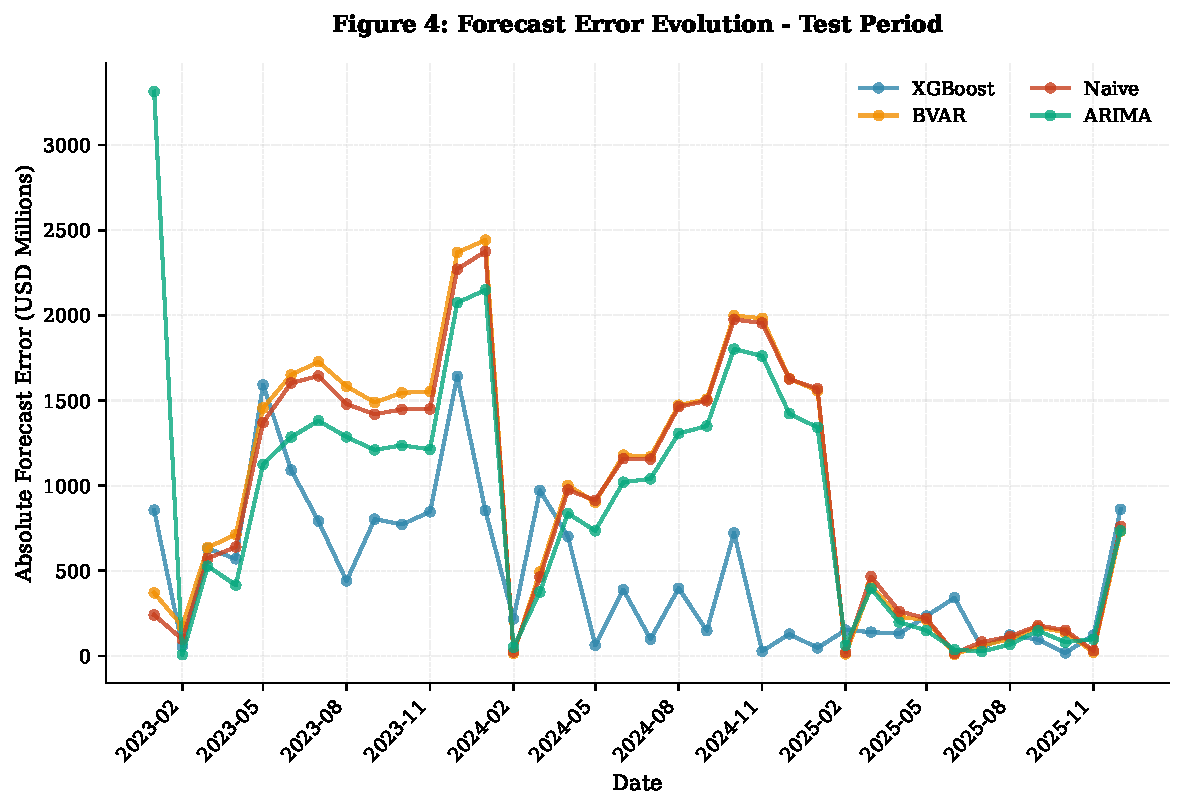
\includegraphics[width=\textwidth]{figures/figure_4_error_decomposition.pdf}
\caption{Absolute forecast errors over the test period (2023--2025) for selected models. MS-VAR maintains consistently lower errors, though all models exhibit episodic spikes corresponding to months of large reserve movements.}
\label{fig:error_decomp}
\end{figure}

\begin{table}[htbp]
\centering
\caption{Crisis Segment Performance: Best Models by Period}
\label{tab:crisis_segment}
\begin{tabular}{llrr}
\toprule
Segment & Best Model & RMSE & Na\"{\i}ve RMSE \\
\midrule
Crisis (2020--2022, BoP validation) & MS-VAR (BoP) & 518.2 & 1345.5 \\
Post-default (2023--2025, BoP test) & MS-VAR (BoP) & 315.2 & 1350.8 \\
All pooled (2020--2025, BoP) & MS-VAR (BoP) & 438.5 & 1338.0 \\
\bottomrule
\end{tabular}
\begin{tablenotes}
\small
\item \textit{Notes:} RMSE values are BoP-specification $h=1$ results from unified rolling-origin outputs. ``All pooled'' combines validation and test forecasts; effective pooled window is 2020:02--2025:03 due BoP data availability.
\end{tablenotes}
\end{table}

The results in Table~\ref{tab:crisis_segment} indicate that the Meese-Rogoff puzzle does not hold in its strong form for reserves. MS-VAR outperforms the na\"{\i}ve random walk during the 2020--2022 validation crisis segment: crisis RMSE of approximately 518 versus na\"{\i}ve crisis RMSE of 1,345, a 61.5\% improvement. This suggests that regime-switching models, when applied to appropriately disaggregated data, can capture reserve depletion dynamics during sudden stops. The result extends beyond the standard Meese-Rogoff finding, which was formulated for exchange rate models applied to aggregated fundamentals.

However, the puzzle retains a weaker form. Among non-regime-switching models, the na\"{\i}ve benchmark remains competitive during crisis periods. None of ARIMA, VECM, BVAR, or XGBoost reliably beats it in the BoP crisis-validation segment. Classical and machine-learning models without explicit regime structure remain vulnerable to abrupt distributional breaks.

\section{Density Forecast Evaluation}

\begin{figure}[htbp]
\centering
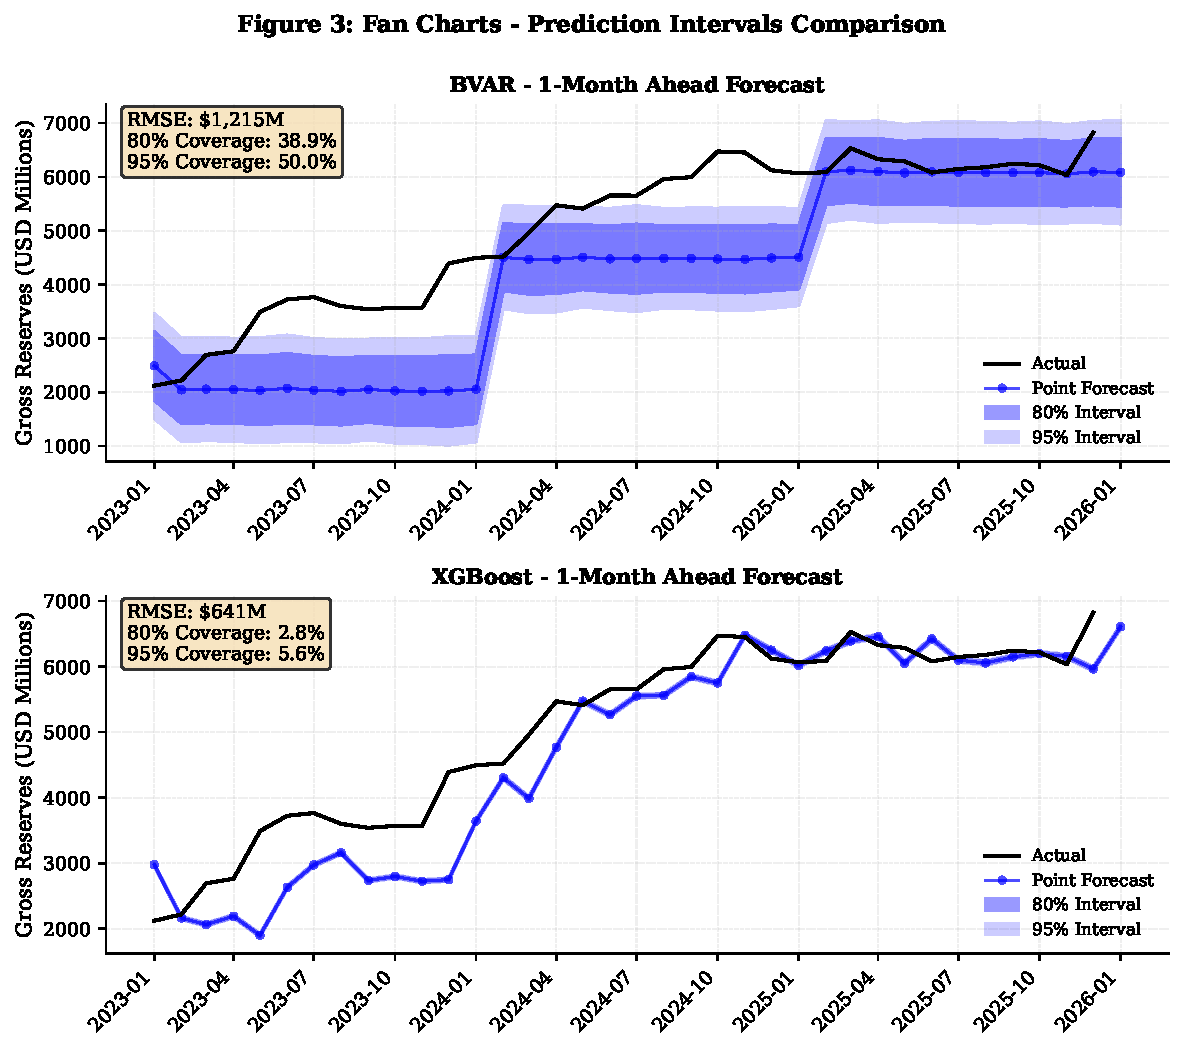
\includegraphics[width=\textwidth]{figures/figure_3_fan_charts.pdf}
\caption{Prediction interval fan charts for BVAR (left) and XGB-Quantile (right). XGB-Quantile produces sharper, better-calibrated intervals; BVAR intervals are wider but exhibit substantial under-coverage relative to nominal levels.}
\label{fig:fan_charts}
\end{figure}

\begin{table}[htbp]
\centering
\caption{Density Forecast Evaluation: Parsimonious Specification, $h = 1$}
\label{tab:density}
\begin{tabular}{lrrrr}
\toprule
Model & CRPS & Log Score & Coverage$_{80}$ (\%) & Coverage$_{95}$ (\%) \\
\midrule
XGB-Quantile & \textbf{241.0} & -- & \textbf{72.2} & \textbf{97.2} \\
XGBoost & 466.4 & $-$928.95 & 2.8 & 5.6 \\
ARIMA & 734.2 & $-$10.12 & 41.7 & 50.0 \\
Na\"{\i}ve & 761.5 & $-$9.88 & 44.4 & 52.8 \\
VECM & 782.4 & $-$10.30 & 36.1 & 52.8 \\
BVAR & 792.1 & $-$10.18 & 38.9 & 50.0 \\
\bottomrule
\end{tabular}
\begin{tablenotes}
\small
\item \textit{Notes:} Coverage$_{80}$ and Coverage$_{95}$ = empirical coverage rates of 80\% and 95\% prediction intervals. Bold indicates best. Models without probabilistic output are marked with dashes.
\end{tablenotes}
\end{table}

Table~\ref{tab:density} evaluates probabilistic forecasting performance. XGB-Quantile is the clear winner, with CRPS of 241.0 and the best coverage rates: 72.2\% at 80\% nominal and 97.2\% at 95\% nominal. Classical specifications (ARIMA, VECM) and BVAR exhibit poor coverage (36--50\% at 80\% nominal), suggesting that their estimated densities substantially underestimate forecast uncertainty---likely because parameter estimates are unstable across regimes. The XGBoost point-forecast model produces extremely narrow implicit intervals (2.8\%/5.6\% coverage). Good point forecasts, in short, do not guarantee good density forecasts.

The implication for policy is a two-model approach: regime-switching models for point forecasting and scenario analysis, complemented by XGB-Quantile or conformal prediction methods for uncertainty quantification.

\section{Scenario Analysis and Robustness}

\subsection{Scenario Analysis}

\begin{table}[htbp]
\centering
\caption{MS-VARX Scenario Analysis: Reserve Projections (Parsimonious)}
\label{tab:scenarios}
\begin{tabular}{lrrrr}
\toprule
Scenario & End Level & $\Delta$ (USD m) & $\Delta$ (\%) \\
\midrule
Combined Upside & 6837.7 & 12.7 & 0.19 \\
Baseline & 6755.7 & $-$69.3 & $-$1.02 \\
Oil Price Shock & 6724.9 & $-$100.1 & $-$1.47 \\
Export Shock ($-$15\%) & 6718.7 & $-$106.3 & $-$1.56 \\
IMF Tranche Delay & 6624.5 & $-$200.5 & $-$2.94 \\
LKR Depreciation 10\% & 6591.7 & $-$233.3 & $-$3.42 \\
Combined Adverse & 6509.7 & $-$315.3 & $-$4.62 \\
LKR Depreciation 20\% & 6427.8 & $-$397.2 & $-$5.82 \\
\bottomrule
\end{tabular}
\begin{tablenotes}
\small
\item \textit{Notes:} Projections based on MS-VARX model with parsimonious specification. 12-month horizon (2025:01--2025:12). Baseline from 2024:12 level of 6,825.0. Remittance and tourism shocks have zero impact under this specification as those variables are excluded; their effects propagate in BoP and fuller specifications.
\end{tablenotes}
\end{table}

Table~\ref{tab:scenarios} presents component-level scenario projections over a 12-month horizon. The baseline projects reserves at 6,755.7 USD million by end-2025, a modest 1.02\% decline. Under a combined adverse scenario (LKR depreciation, export shock, oil price spike, IMF disbursement delay), reserves decline to 6,509.7 million ($-$4.62\%), while a 20\% currency depreciation alone produces a 5.82\% decline. IMF disbursement delays prove particularly consequential ($-$2.94\%), underscoring the sensitivity of the recovery trajectory to programme timing.

Variable set sensitivity analysis reveals that the full specification is most vulnerable to adverse shocks (9.97\% decline under combined adverse in the full specification), whilst the parsimonious specification is most stable (4.62\%). The BoP specification uniquely captures remittance decline impacts ($-$3.78\%) and tourism recovery effects (+0.89\%) that are invisible in the parsimonious system.

\subsection{Robustness to Train/Test Split}

\begin{table}[htbp]
\centering
\caption{Split Robustness: RMSE and Rank by Train/Validation Partition (BoP, $h=1$)}
\label{tab:split_robustness}
\begin{tabular}{lrrr|rr}
\toprule
& \multicolumn{3}{c}{RMSE by Split} & \multicolumn{2}{c}{Rank Statistics} \\
\cmidrule(lr){2-4} \cmidrule(lr){5-6}
Model & Baseline & Early & Late & Avg.\ Rank & Rank SD \\
\midrule
MS-VAR & 315.2 & 275.9 & 260.6 & 1.00 & 0.00 \\
DMA & 321.7 & 282.9 & 264.5 & 2.33 & 0.58 \\
MS-VECM & 323.4 & 291.4 & 268.9 & 3.33 & 0.58 \\
DMS & 326.0 & 285.4 & 260.6 & 2.67 & 1.53 \\
XGBoost & 886.1 & 1115.0 & 623.5 & 5.00 & 0.00 \\
\bottomrule
\end{tabular}
\begin{tablenotes}
\small
\item \textit{Notes:} Baseline split: train to 2019-12, validate to 2022-12. Early split: train to 2018-12, validate to 2021-12. Late split: train to 2020-12, validate to 2023-12. DMS ties MS-VAR in the late split (260.6). The split-robust evaluation set excludes LSTM and BoPIdentity (configuration flags `include\_lstm = false`, `include\_bop = false`); the table therefore reports the top five models within that evaluated set. Remaining evaluated models (ARIMA, Na\"{\i}ve, BVAR, VECM) have RMSE $>$ 1,200 in all splits.
\end{tablenotes}
\end{table}

Table~\ref{tab:split_robustness} addresses whether the model ranking is an artefact of a particular train/validation/test partition. Under three split definitions (baseline: train to 2019-12, validate to 2022-12; early: 2018-12/2021-12; late: 2020-12/2023-12), MS-VAR holds rank 1 in every case. The corresponding RMSEs are 315.2, 275.9, and 260.6. Its average rank is 1.00 with zero rank variance.

DMA is the most stable runner-up (average rank 2.33, rank SD 0.58). DMS ties MS-VAR in the late split at 260.6 but is less stable overall (average rank 2.67, rank SD 1.53). The gap between the top-four cluster and XGBoost widens in the early split, where XGBoost deteriorates to 1,115.0, nearly four times the MS-VAR error.

These results support two claims. First, the gains from regime-switching architecture are genuine, not driven by a favourable partition. Second, stability and accuracy are distinct properties. Some simpler models (e.g., Na\"{\i}ve) are relatively stable across splits but at worse loss levels. The regime-aware models are both accurate and stable, which is uncommon in macroeconomic forecasting comparisons \citep{Rossi2013}.

Split choice does, however, materially affect regime diagnostics. The training-validation subsample converged where the full-sample estimation often did not, and estimated regime durations differ across splits. Production forecasting systems should report results across multiple configurations and flag cases where regime diagnostics are qualitatively different.

\section{Conclusion}

This paper compares classical econometric, Bayesian, regime-switching, and machine learning models for forecasting Sri Lanka's foreign exchange reserves. The evaluation spans five variable sets, multiple forecast horizons, and a dataset encompassing stable accumulation, pandemic disruption, sovereign default, and IMF-supervised recovery. Beyond the model comparison, the analysis introduces a factorial architecture-versus-information decomposition and provides analytical evidence for the sources of regime-switching forecast advantage.

The central result is the strong performance of regime-aware methods. MS-VAR achieves RMSE reductions of roughly three-quarters relative to the na\"{\i}ve benchmark. DMA and DMS perform nearly as well, and the 90\% Model Confidence Set retains all four regime-aware specifications while eliminating all others. This ranking is stable across three alternative train/test splits. The 2$\times$2 factorial decomposition shows that the advantage is primarily architectural: regime-switching structure accounts for the bulk of the improvement over gradient-boosted trees. The interaction term indicates that architecture and information content are complements for regime-switching models but substitutes for tree-based methods.

The information-loss analysis demonstrates that aggregating balance-of-payments flows destroys the majority of the available signal through cancellation of offsetting gross flows. Regime characterisation reveals highly persistent states with near-perfect classification certainty. Impulse response analysis shows regime asymmetry in shock propagation consistent with distinct crisis and recovery dynamics.

The Meese-Rogoff puzzle does not hold in its strong form for reserves. MS-VAR outperforms the na\"{\i}ve benchmark even during the acute crisis segment. A weaker form persists: among non-regime-switching models, the random walk remains competitive during crisis periods. XGBoost dominates in the monetary and full specifications, suggesting that tree models can exploit broader nonlinear feature spaces when dimensionality is sufficient. However, their reliance on autoregressive reserve features limits their ability to exploit structural BoP information.

\subsection{Limitations and Future Work}

Several limitations circumscribe these findings. First, although seeded multi-start checks indicate local stability around the baseline MS-VAR solution, broader random initialisations can still locate inferior local optima. Regime estimation in short samples therefore remains non-trivial and should always be accompanied by reported convergence diagnostics. Second, LSTM robustness remains incompletely explored. Recurrent architectures are sensitive to sequence length, learning rate, and regularisation. More exhaustive tuning could alter the relative ranking of neural network approaches. Third, the single-country design limits generalisability. Application to a cross-country panel of emerging markets, particularly those with different external vulnerability profiles, would test whether the MS-VAR advantage is specific to Sri Lanka or reflects a more general property. Fourth, real-time data vintage effects are not explicitly modelled. The use of revised data may overstate forecast accuracy relative to what would have been achievable in real time.

Several avenues for future research emerge. Conformal prediction methods offer a principled approach to combining regime-switching point-forecast accuracy with distribution-free uncertainty quantification. Such methods could resolve the gap between MS-VAR's point forecast advantage and XGB-Quantile's superior density calibration. Ensemble methods combining regime-switching models with machine learning via stacking could exploit complementary strengths: structural regime identification from MS-VAR and flexible nonlinear feature extraction from tree-based methods. Finally, extending the information-loss framework to other macroeconomic aggregates (GDP components, monetary aggregates) would test whether the cancellation documented here for balance-of-payments flows is a broader phenomenon.

Despite these limitations, the evidence consistently favours regime-aware approaches. Explicitly modelling regime dynamics in disaggregated balance-of-payments systems appears strongly beneficial for reserve forecasting in crisis-prone emerging markets, though the single-country design means this conclusion should be tested in other settings. Central banks confronted with reserve surveillance should consider pairing regime-switching models for scenario analysis with complementary probabilistic methods for uncertainty quantification.

\bibliographystyle{plainnat}
\begin{thebibliography}{99}

\bibitem[Aizenman, 2012]{Aizenman2012}
Aizenman, J. (2012).
\newblock The internationalization of the RMB, capital market openness, and financial reforms in China.
\newblock \textit{Pacific Economic Review}, 17(3):321--338.

\bibitem[Aizenman and Lee, 2007]{AizenmanLee2007}
Aizenman, J. and Lee, J. (2007).
\newblock International reserves: precautionary versus mercantilist views, theory and evidence.
\newblock \textit{Open Economies Review}, 18(2):191--214.

\bibitem[Athukorala, 2024]{Athukorala2024}
Athukorala, P. (2024).
\newblock Sri Lanka's external sector crisis: causes and consequences.
\newblock \textit{World Development}, 177:106556.

\bibitem[Banbura et al., 2010]{Banbura2010}
Banbura, M., Giannone, D., and Reichlin, L. (2010).
\newblock Large Bayesian vector auto regressions.
\newblock \textit{Journal of Business \& Economic Statistics}, 28(1):57--75.

\bibitem[Brunetti et al., 2007]{BrunettiMarianoScottiTan2007}
Brunetti, C., Mariano, R. S., Scotti, C., and Tan, A. H. (2007).
\newblock Markov switching and stochastic volatility in currency crises.
\newblock \textit{Journal of Applied Econometrics}, 22(4):765--789.

\bibitem[Calvo, 1996]{Calvo1996}
Calvo, G. A. (1996).
\newblock Varieties of capital flows and their implications for the economy.
\newblock In \textit{The Economic of Globalization: Policy Perspectives from the East Asia and Pacific}, pages 15--41. World Bank, Washington, DC.

\bibitem[Calvo, 1998]{Calvo1998}
Calvo, G. A. (1998).
\newblock Contagion, well-behavedness and sudden stops.
\newblock \textit{NBER Working Paper No. 5854}.

\bibitem[Calvo et al., 2013]{CalvoIzquierdoLooKung2013}
Calvo, G. A., Izquierdo, A., and Loo-Kung, R. (2013).
\newblock Optimal holdings of international reserves: self-insurance against sudden stops.
\newblock \textit{Journal of International Economics}, 87(2):266--286.

\bibitem[Carriero et al., 2015]{Carriero2015}
Carriero, A., Clark, T. E., and Marcellino, M. (2015).
\newblock Realizing the gains from Bayesian dynamic model averaging.
\newblock \textit{International Journal of Forecasting}, 31(4):1009--1023.

\bibitem[CBSL Annual Report, 2021]{CBSLAnnualReport2021}
Central Bank of Sri Lanka (2021).
\newblock Annual Report 2021.
\newblock Central Bank of Sri Lanka, Colombo.

\bibitem[Chen and Guestrin, 2016]{ChenGuestrin2016}
Chen, T. and Guestrin, C. (2016).
\newblock XGBoost: A scalable tree boosting system.
\newblock In \textit{Proceedings of the 22nd ACM SIGKDD International Conference on Knowledge Discovery and Data Mining}, pages 785--794. ACM.

\bibitem[Cheung et al., 2005]{CheungChinnPascual2005}
Cheung, Y. W., Chinn, M. D., and Pascual, A. G. (2005).
\newblock Empirical exchange rate models of the nineties: Are any fit to survive?
\newblock \textit{Journal of International Money and Finance}, 24(7):1150--1175.

\bibitem[Doan et al., 1984]{DoanLittermanSims1984}
Doan, T. A., Litterman, R. B., and Sims, C. A. (1984).
\newblock Forecasting and conditional projection using realistic prior distributions.
\newblock \textit{Econometric Reviews}, 3(1):1--100.

\bibitem[Diebold and Mariano, 1995]{DieboldMariano1995}
Diebold, F. X. and Mariano, R. S. (1995).
\newblock Comparing predictive accuracy.
\newblock \textit{Journal of Business \& Economic Statistics}, 13(3):253--263.

\bibitem[Frankel and Saravelos, 2012]{FrankelSaravelos2012}
Frankel, J. A. and Saravelos, G. (2012).
\newblock Can we predict the next financial crisis?
\newblock \textit{NBER Working Paper No. 18725}.

\bibitem[Ghosh et al., 2017]{Ghosh2017}
Ghosh, A. R., Ostry, J. D., and Qureshi, M. S. (2017).
\newblock Taming the tide of capital flows: a policy guide.
\newblock \textit{Journal of International Economics}, 105:S22--S38.

\bibitem[Gosselin and Parent, 2005]{Gosselin2005}
Gosselin, M.-A. and Parent, N. (2005).
\newblock An empirical analysis of foreign exchange reserves in emerging Asia.
\newblock \textit{Bank of Canada Working Paper No. 2005-38}.

\bibitem[Greenspan, 1999]{Greenspan1999}
Greenspan, A. (1999).
\newblock Currency reserves and debt.
\newblock \textit{Remarks before the World Bank Conference on Recent Trends in Reserves Management}, Washington, DC.

\bibitem[Gupta et al., 2014]{Gupta2014}
Gupta, R., Hammoudeh, S., Kim, W. J., and Simo-Kengne, B. D. (2014).
\newblock Forecasting China's foreign exchange reserves using dynamic model averaging: the roles of macroeconomic fundamentals, financial stress and economic uncertainty.
\newblock \textit{The North American Journal of Economics and Finance}, 28:323--336.

\bibitem[Hamilton, 1989]{Hamilton1989}
Hamilton, J. D. (1989).
\newblock A new approach to the economic analysis of nonstationary time series and the business cycle.
\newblock \textit{Econometrica}, 57(2):357--384.

\bibitem[Hansen et al., 2011]{HansenLundeNason2011}
Hansen, P. R., Lunde, A., and Nason, J. M. (2011).
\newblock The model confidence set.
\newblock \textit{Econometric Reviews}, 30(2):160--201.

\bibitem[Hochreiter and Schmidhuber, 1997]{HochreiterSchmidhuber1997}
Hochreiter, S. and Schmidhuber, J. (1997).
\newblock Long short-term memory.
\newblock \textit{Neural Computation}, 9(8):1735--1780.

\bibitem[Hyndman and Koehler, 2006]{HyndmanKoehler2006}
Hyndman, R. J. and Koehler, A. B. (2006).
\newblock Another look at measures of forecast accuracy.
\newblock \textit{International Journal of Forecasting}, 22(4):679--688.

\bibitem[IMF, 2011]{IMF2011}
IMF (2011).
\newblock Assessing reserve adequacy.
\newblock \textit{IMF Policy Paper}.

\bibitem[IMF, 2015]{IMF2015}
IMF (2015).
\newblock Assessing reserve adequacy---review of the adequacy approach.
\newblock \textit{IMF Policy Paper}.

\bibitem[IMF, 2022]{IMF2022}
IMF (2022).
\newblock Sri Lanka: Request for an extended arrangement under the Extended Fund Facility.
\newblock \textit{IMF Country Report No. 23/99}.

\bibitem[Jeanne and Ranci\`{e}re, 2011]{JeanneRanciere2011}
Jeanne, O. and Ranci\`{e}re, R. (2011).
\newblock The optimal level of international reserves for emerging market countries.
\newblock \textit{Journal of International Economics}, 85(2):229--240.

\bibitem[Johansen, 1988]{Johansen1988}
Johansen, S. (1988).
\newblock Statistical analysis of cointegration vectors.
\newblock \textit{Journal of Economic Dynamics and Control}, 12(2-3):231--254.

\bibitem[Johansen, 1991]{Johansen1991}
Johansen, S. (1991).
\newblock Estimation and hypothesis testing of cointegration vectors in Gaussian vector autoregressive models.
\newblock \textit{Econometrica}, 59(6):1551--1580.

\bibitem[Kaminsky et al., 1998]{KaminskyLizondoReinhart1998}
Kaminsky, G. L., Lizondo, S., and Reinhart, C. M. (1998).
\newblock Leading indicators of currency crises.
\newblock \textit{IMF Staff Papers}, 45(1):1--48.

\bibitem[Koop and Korobilis, 2012]{KoopKorobilis2012}
Koop, G. and Korobilis, D. (2012).
\newblock Forecasting inflation using dynamic model averaging.
\newblock \textit{International Economic Review}, 53(3):867--886.

\bibitem[Krolzig, 1997]{Krolzig1997}
Krolzig, H. M. (1997).
\newblock \textit{Markov-Switching Vector Autoregressions: Modelling, Statistical Inference, and Application to Business Cycle Analysis}.
\newblock Springer, Berlin.

\bibitem[Litterman, 1986]{Litterman1986}
Litterman, R. B. (1986).
\newblock Forecasting with Bayesian vector autoregressions---five years of experience.
\newblock \textit{Journal of Business \& Economic Statistics}, 4(1):25--38.

\bibitem[Medeiros et al., 2021]{MedeirosVasconcelosVeigaZilberman2021}
Medeiros, M. C., Vasconcelos, G. F., Veiga, \'{A}., and Zilberman, E. (2021).
\newblock Forecasting inflation in a data-rich environment: the benefits of machine learning methods.
\newblock \textit{Journal of Business \& Economic Statistics}, 39(1):98--119.

\bibitem[Meese and Rogoff, 1983]{MeeseRogoff1983}
Meese, R. A. and Rogoff, K. (1983).
\newblock Empirical exchange rate models of the seventies: Do they fit out of sample?
\newblock \textit{Journal of International Economics}, 14(1-2):3--24.

\bibitem[Obstfeld et al., 2010]{Obstfeld2010}
Obstfeld, M., Shambaugh, J. C., and Taylor, A. M. (2010).
\newblock Financial stability and the global safeguard system.
\newblock In \textit{NBER International Seminar on Macroeconomics 2009}, pages 9--37. University of Chicago Press.

\bibitem[Peria, 2002]{Peria2002}
Peria, M. S. M. (2002).
\newblock A regime-switching approach to speculative attacks: a focus on European currencies.
\newblock \textit{Journal of International Economics}, 57(2):467--490.

\bibitem[Raftery et al., 2010]{Raftery2010}
Raftery, A. E., K\'{a}rn\'{y}, M., and Ettler, P. (2010).
\newblock Online prediction under model uncertainty via dynamic model averaging: application to a cold rolling mill.
\newblock \textit{Technometrics}, 52(2):52--66.

\bibitem[Richardson et al., 2021]{RichardsonMulderVehbi2021}
Richardson, A., Mulder, T., and Vehbi, T. (2021).
\newblock Nowcasting New Zealand GDP using machine learning algorithms.
\newblock \textit{International Journal of Forecasting}, 37(2):736--759.

\bibitem[Sehgal and Sharma, 2008]{SehgalSharma2008}
Sehgal, S. and Sharma, C. (2008).
\newblock A study of adequacy, cost and determinants of international reserves in India.
\newblock \textit{International Research Journal of Finance and Economics}, 20:7--21.

\bibitem[Rossi, 2013]{Rossi2013}
Rossi, B. (2013).
\newblock Exchange rate predictability.
\newblock \textit{Journal of Economic Literature}, 51(4):1063--1119.

\bibitem[Salas et al., 2025]{Salas2025}
Salas, S., Hernandez-del-Valle, G., and Elizondo, R. (2025).
\newblock Forecasting foreign exchange reserves using Bayesian model averaging and na\"{\i}ve Bayes classification.
\newblock \textit{International Journal of Forecasting}, forthcoming.

\bibitem[Sims, 1980]{Sims1980}
Sims, C. A. (1980).
\newblock Macroeconomics and reality.
\newblock \textit{Econometrica}, 48(1):1--48.

\bibitem[Taylor et al., 2001]{TaylorPeelSarno2001}
Taylor, M. P., Peel, D. A., and Sarno, L. (2001).
\newblock Nonlinear mean-reversion in real exchange rates: towards a solution to the purchasing power parity puzzles.
\newblock \textit{International Journal of Finance \& Economics}, 6(4):299--318.

\bibitem[Yu et al., 2007]{Yu2007}
Yu, L., Wang, S., and Lai, K. K. (2007).
\newblock Foreign-exchange-rate forecasting with artificial neural networks.
\newblock \textit{International Series in Operations Research \& Management Science}, 107.

\bibitem[UNDP, 2022]{UNDP2022}
UNDP (2022).
\newblock The Sri Lankan economic crisis: impacts and policy responses.
\newblock \textit{UNDP Sri Lanka Report}.

\bibitem[Weerakoon and Jayasuriya, 2023]{Weerakoon2023}
Weerakoon, D. and Jayasuriya, S. (2023).
\newblock The political economy of Sri Lanka's debt crisis.
\newblock \textit{South Asia: Journal of South Asian Studies}, 46(1):123--145.

\bibitem[Wijnholds and Kapteyn, 2001]{Wijnholds2001}
Wijnholds, J. O. and Kapteyn, A. (2001).
\newblock Reserve adequacy in emerging market economies.
\newblock \textit{IMF Working Paper WP/01/143}.

\end{thebibliography}

\appendix

\section{Estimation Details and Metric Definitions}

\subsection{Classical Models}

ARIMA models with exogenous regressors are estimated via maximum likelihood, with lag order selected via AIC across ARIMA($p,d,q$) specifications with $p, q \in \{0,1,2,3\}$ and $d \in \{0,1\}$. VAR and VECM models are estimated via full-information maximum likelihood with lag order selected by AIC (maximum 4 lags). Cointegration rank is determined by the Johansen trace and maximum eigenvalue tests.

\subsection{Bayesian VAR}

The BVAR Minnesota prior is centred on a random walk with hyperparameters: overall shrinkage $\lambda \in [0.1, 1.5]$, lag decay $\mu \in [0.1, 0.8]$, and own-lag variance $\phi \in [0.1, 0.95]$, selected via grid search on in-sample BIC. The posterior is simulated via Gibbs sampling with 10,000 draws (2,000 burn-in).

\subsection{Machine Learning}

XGBoost: 200 boosting rounds (300 for BoP), learning rate $\eta = 0.1$, tree depth 3--5, minimum child weight 1, subsample ratio 0.8--1.0, column subsample 0.8, time-series cross-validation. Features include lagged dependent variable (lags 1--12), lagged exogenous variables (lags 1--6), and rolling 3- and 6-month means and volatilities.

LSTM: single recurrent layer of 64 units, input sequence length 12, Adam optimiser (learning rate 0.001), dropout 0.2, batch size 32, maximum 100 epochs with early stopping (patience 10).

\subsection{Accuracy Metrics}

\begin{align}
\text{RMSE} &= \sqrt{\frac{1}{n} \sum_{t=1}^{n} (y_t - \hat{y}_t)^2} \\
\text{MAE} &= \frac{1}{n} \sum_{t=1}^{n} |y_t - \hat{y}_t| \\
\text{MAPE} &= \frac{100}{n} \sum_{t=1}^{n} \left| \frac{y_t - \hat{y}_t}{y_t} \right| \\
\text{MASE} &= \text{MAE} \bigg/ \frac{1}{n-1} \sum_{t=2}^{n} |y_t - y_{t-1}|
\end{align}

The asymmetric policy loss function is defined as:
\[
L(e_t) = \begin{cases} 2 \cdot e_t^2 & \text{if } e_t < 0 \text{ (under-prediction)} \\ e_t^2 & \text{if } e_t \geq 0 \text{ (over-prediction)} \end{cases}
\]

Probabilistic forecast metrics:
\begin{align}
\text{CRPS} &= \frac{1}{n} \sum_{t=1}^{n} \int_{-\infty}^{\infty} [F_t(z) - \mathbf{1}_{z \geq y_t}]^2 \, dz \\
\text{Log score} &= \log p_t(y_t)
\end{align}

The Diebold-Mariano statistic is $\text{DM} = \bar{d} / \sqrt{2\pi f_d(0) / n}$, which is asymptotically standard normal under the null of equal expected loss.

\end{document}
